\documentclass[12pt,prb,aps,epsf]{article}
\usepackage[utf8]{inputenc}
\usepackage{amsmath}
\usepackage{amsfonts}
\usepackage{amssymb}
\usepackage{graphicx} 
\usepackage{latexsym} 
\usepackage[toc,page]{appendix}
\usepackage{listings}
\usepackage{xcolor}
\usepackage{soul}
\usepackage[T1]{fontenc}
\usepackage{amsthm}
\usepackage{mathtools}
\usepackage{setspace}
\usepackage{array,multirow,makecell}
\usepackage{geometry}
\usepackage{textcomp}
\usepackage{float}
%\usepackage{siunitx}
\usepackage{cancel}
%\usepackage{tikz}
%\usetikzlibrary{calc, shapes, backgrounds, arrows, decorations.pathmorphing, positioning, fit, petri, tikzmark}
\usepackage{here}
\usepackage{titlesec}
%\usepackage{bm}
\usepackage{bbold}

\geometry{hmargin=2cm,vmargin=2cm}

\begin{document}
	
	\title{MP 06 Transition de phase}
	\author{Maria}
	
	\maketitle
	
	\tableofcontents
	
	\pagebreak
	
	
\section{Chaleur latente de vaporisation de l'eau}
On chauffe de l'eau dans un calorimètre avec une grosse résistance, et on mesure la puissance fournie avec un puissancemètre. Une fois arrivé à ébullition (on mesure la température de l'eau avec une résistance de platine pour s'en assurer) on note la masse totale calorimètre + eau, puis on lance le chrono. On note ensuite la variation de masse observée à chaque intervalle de temps $\Delta t$, et on trace alors $m_n(n\Delta t)$, que l'on peut alors modéliser par une droite, car on a 
\begin{eqnarray}
Q = L_v\Delta m = P \Delta t
\end{eqnarray}
par définition de la chaleur latente. On en déduit alors 
\begin{eqnarray}
L_v = P\frac{\Delta t}{\Delta m} = \frac{P}{a}
\end{eqnarray} 
avec $a$ le coefficient directeur de la droite obtenue.\\
On a, pour les incertitudes 
\begin{eqnarray}
\frac{u(L_v)}{L_v} = \sqrt{\left(\frac{u(P)}{P}\right)^2 + \left(\frac{u(a)}{a}\right)^2}
\end{eqnarray}
où $\frac{u(P)}{P} = 1\%$ est donné par la notice du puissancemètre.\\
On obtient ici $L_v = 2270\pm 27$ kJ.kg$^{-1}$ (pour une puissance de 404 W) que l'on peut alors comparer avec la valeur tabulé $L_v^{tab} = 2257$ kJ.kg$^{-1}$.\\

\textbf{Remarque} : on place un sèche cheveux au dessus du calorimètre pour évacuer efficacement la vapeur d'eau.\\
\textbf{Remarque} : Il faut se placer à 400-500 W pour une utilisation optimale du puissancemètre.\\
\textbf{Remarque} : Si possible on peut mettre la potence portant la résistance sur la balance pour s'affranchir de la poussée d'Archimède, donc demander une potence en bois.

\begin{figure}
	\centerline{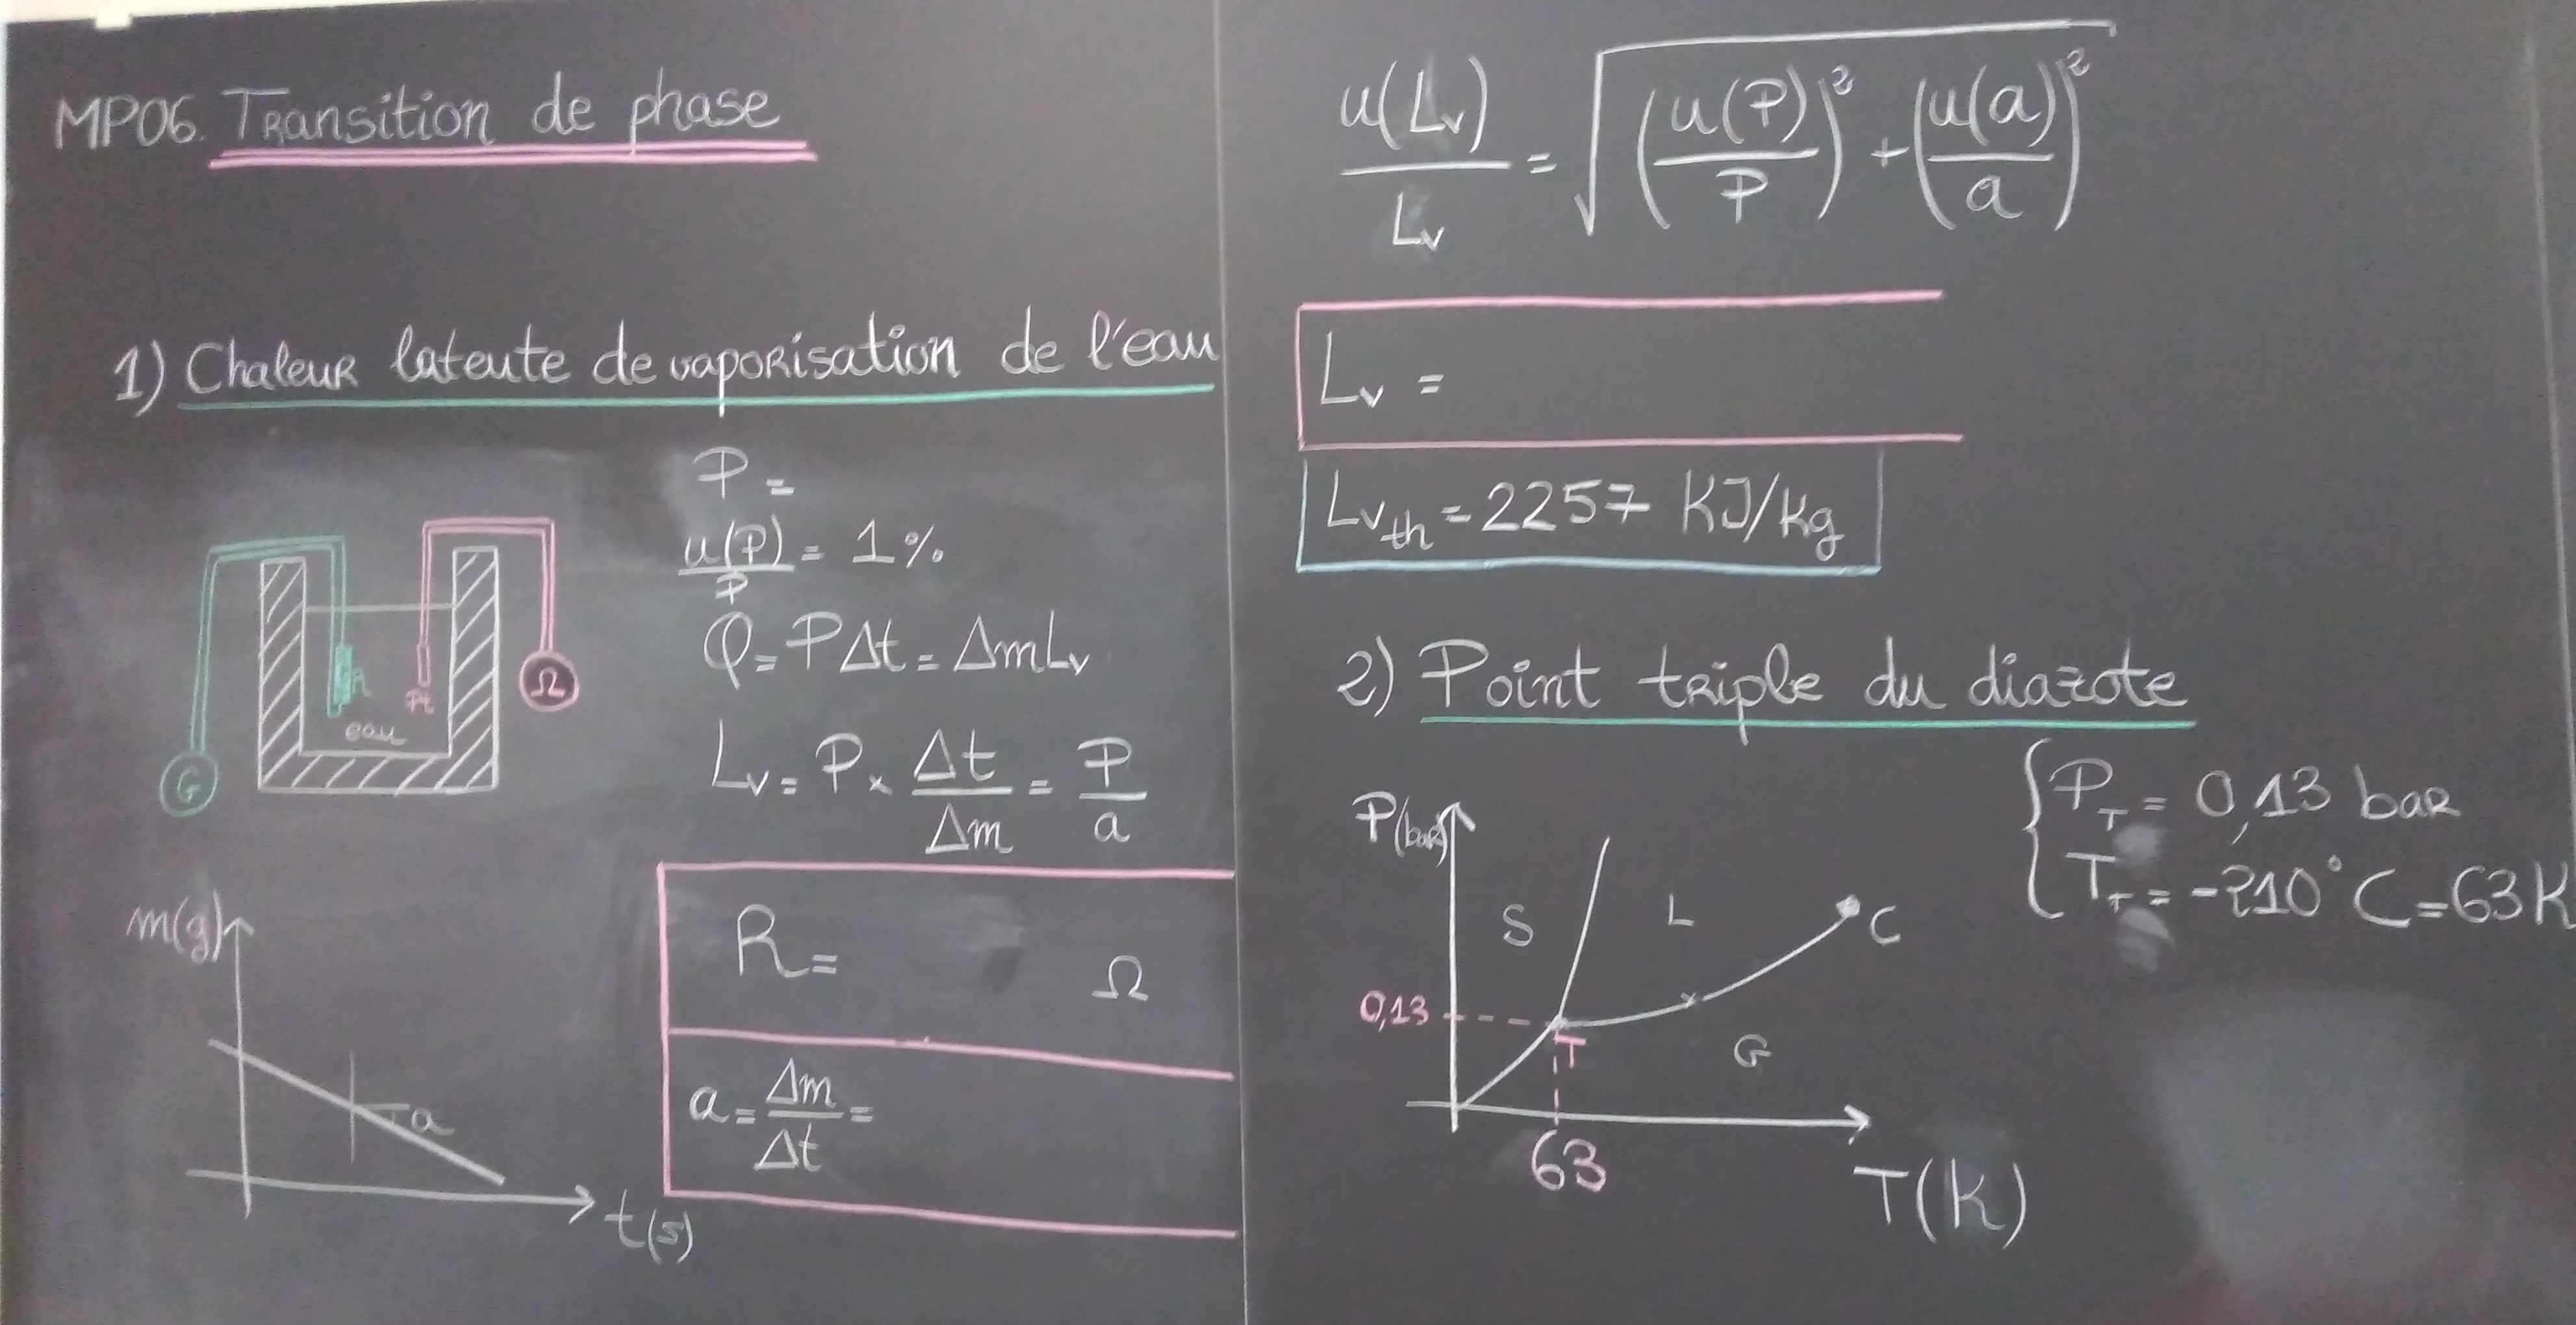
\includegraphics[width=15cm]{T1}}
\end{figure}

\section{Point triple du diazote}
\begin{figure}
	\centerline{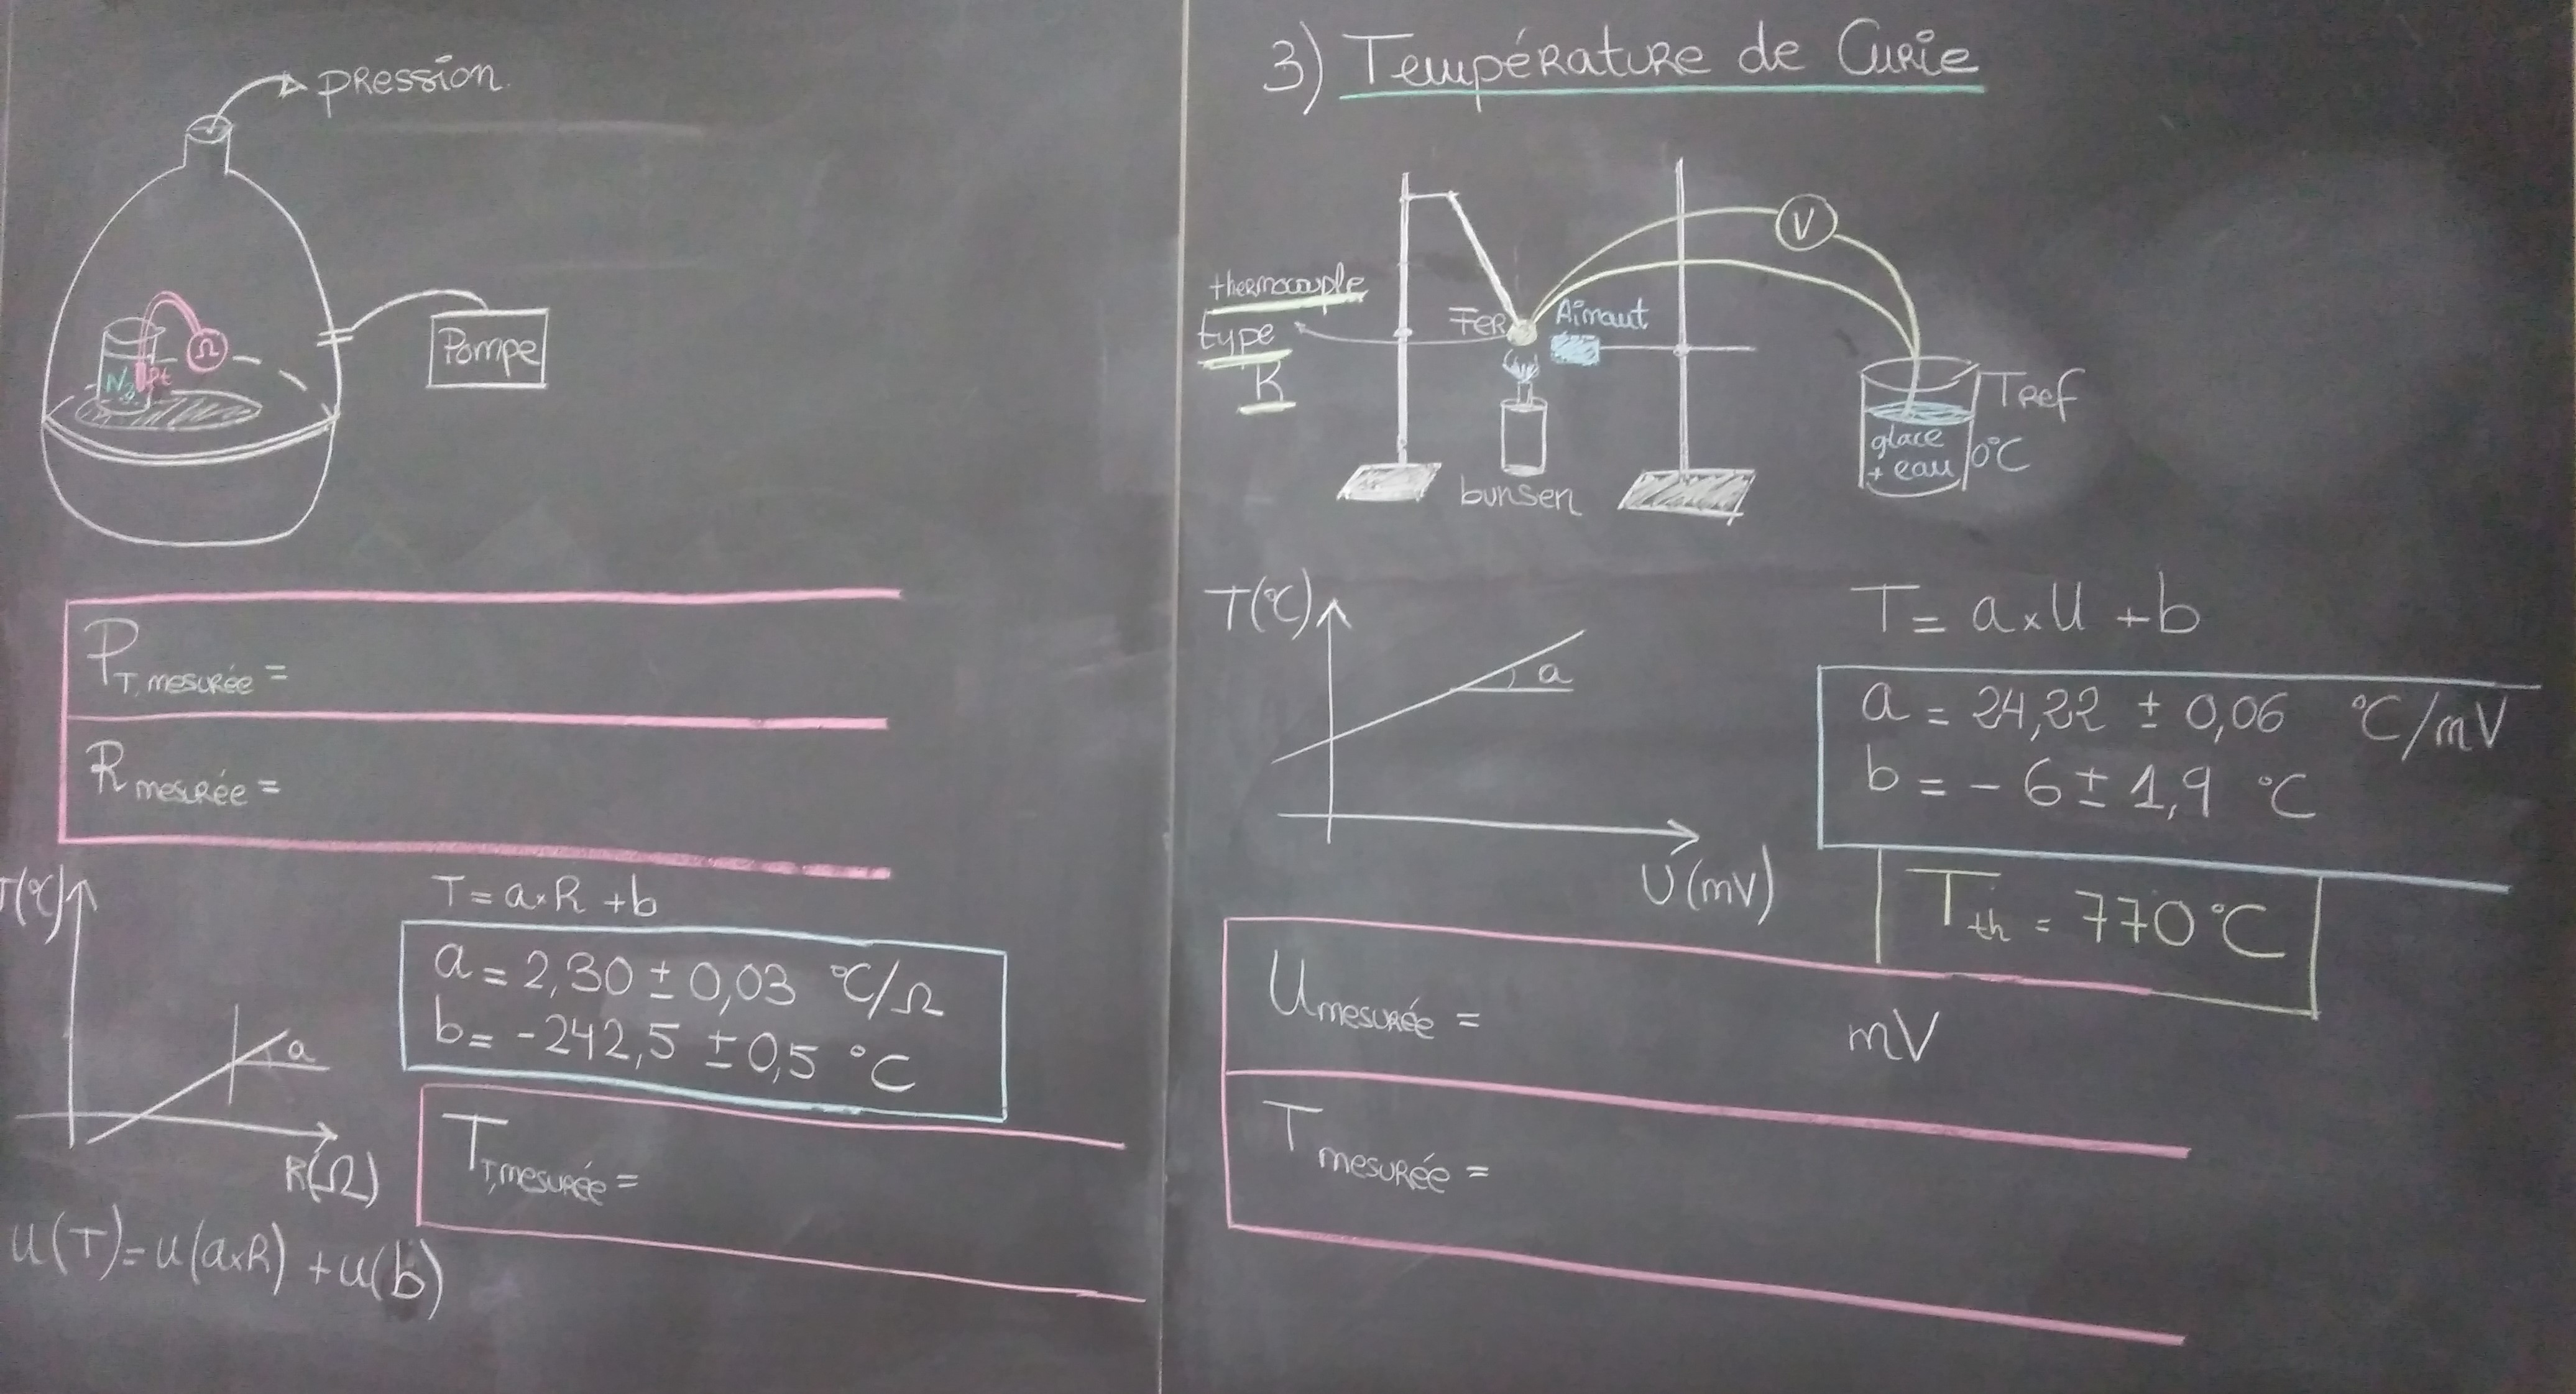
\includegraphics[width=18cm]{T2}}
\end{figure}

La position du point triple de l'azote est tabulé à 
\begin{eqnarray}
P_T = 0.13\,bar\\
T_T = -210^oC = 63\,K
\end{eqnarray}
On va s'y placer ici grâce au dispositif représenté sur la photo; on utilise de l'azote liquide que l'on verse dans un bêcher, qui est lui même placé dans une cuve dans laquelle on peut diminuer la pression à l'aide d'une pompe. Un manomètre fixé sur la cuve permet de connaître la valeur de la pression, et on place une sonde de platine dans la cuve pour contrôler la température de l'azote. On diminue la pression jusqu'à voir apparaître les trois phases simultanément, signe qu'on a atteint le point triple.\\

Ici on mesure 
\begin{eqnarray}
P_T^{mes} = 0.14\, bar\\
R_{Pt} = 15.6\pm 0.1\, \Omega
\end{eqnarray}
On a étalonné la résistance de platine, ce qui permet de donner $T_T^{mes} = -206.62^oC$.\\

\textbf{Remarque} : Il faut mettre assez d'azote, car il s'évapore et part dans la pompe, il en faut donc assez pour que lorsqu'on arrive au point triple la sonde de platine trempe encore.

\section{Température de Curie}	
On attire un pendule en fer par un aimant, qui incline donc le pendule. On chauffe ensuite le bout (en fer) du pendule avec un bec bunsen, et on mesure la température à l'aide d'un thermocouple. Lorsque le fer est porté à la température de Curie le pendule cesse d'être attiré et chute alors. On note cette température (Dans la pratique on note la tension liée au thermocouple, à laquelle on associe une température grâce à l'étalonnage réalisé), que l'on peut ensuite comparer à la température de Curie tabulé $T_{Curie}^{tab} = 770$°C. Ici on a obtenu $T_{Curie} = 752.1$°C.

\section*{Questions}
Pourquoi le fer est il attiré par l'aimant ?\\

Y a t'il une chaleur latente pour la transition ferro-para ?\\
Non car c'est une transition de phase du deuxième ordre.\\

Dans ce montage les transitions sont de quel ordre ?\\

Pour la température de Curie, s'attend on à mesurer une température de Curie plus faible ou plus grande que la température tabulé ?\\
Plus faible, car le morceau de fer n'est pas collé à l'aimant.\\

Quel est le critère pour évaluer si on a atteint le point triple ?\\
On observe du liquide, du solide et de la vapeur simultanément. De plus la température et la pression arrêtent de varier.\\

Quel est l'intérêt de montrer un point triple ? \\
Le Kelvin est défini à partir du point triple de l'eau.\\

Pouvez vous mesurer, là en direct, la capacité calorifique de l'eau ?\\
Oui, de manière similaire à la première manip : on chauffe en contrôlant la puissance, on mesure la masse d'eau (à priori constante, enlever la résistance sinon poussée d'Archimède), et on note la température tous les $\Delta t$. On trace ensuite $T_n(n\Delta t)$, que l'on modélise par une droite, la capacité calorifique étant définie comme 
\begin{eqnarray}
Q = P\Delta t = mc_p\Delta T
\end{eqnarray}

Pourquoi la résistance de platine varie t'elle avec la température ?\\
Collisions électrons-phonons : le nombre de collisions augmente avec la température, engendrant une augmentation de la résistance.

\section*{Remarques}
Il n'y a qu'une courbe dans ce montage, deux manip ne font qu'un point de mesure.\\
On peut lancer direct le chauffage (pour la 1ere manip) au tout début du montage pour gagner du temps.\\

On peut aussi faire la mesure de la température de fusion de l'étain, où on peut montrer le phénomène de surfusion.\\

Manip de transition vers le supra possible : on trempe une plaquette dans l'azote, on mesure sa température avec un thermocouple, et on mesure en même temps la résistance. On trace ensuite $R(T)$.\\

Il faut donner les températures en Kelvin, et modéliser directement en Kelvin.

\end{document}